\documentclass[12pt]{article}

\usepackage{amsmath}
\usepackage{graphicx}
\usepackage{booktabs}
\usepackage{setspace}
\usepackage{geometry}

\geometry{margin=1in}
\onehalfspacing

\title{Replication and Extension of Jealousy Responses to Rival Characteristics}
\author{}
\date{}

\begin{document}
	
	\maketitle
	
	\section*{Abstract}
	This report replicates a 2020 evolutionary psychology study on jealousy responses to romantic rivals and extends the analysis in two ways. The original study examined whether men and women respond differently to rival attractiveness and rival dominance, with particular attention to the interaction between rival attractiveness and participant gender. Using the authors’ publicly available data and code structure, I reproduced the main jealousy models for Study 1 and Study 2. 
	
	I then implemented two extensions. First, I conducted a direct cross-study robustness comparison of the \textit{Attractive condition $\times$ Gender} interaction. Second, I re-estimated the core relationship using an ordered logit model, which is more appropriate for ordinal jealousy measures. 
	
	The results show that the attractiveness-by-gender pattern is strongest in Study 1 and weaker in Study 2. The ordered logit analysis broadly supports the same interpretation but suggests that the magnitude and stability of the effect are limited. Overall, the replication confirms the original findings only partially and shows sensitivity to both sample and model specification.
	
	\section{Introduction}
	Jealousy is a central topic in evolutionary psychology, often interpreted as an adaptive response to threats to romantic relationships. One influential claim is that men and women respond differently to types of romantic rivals. In particular, women may respond more strongly to rival attractiveness, whereas men may respond more strongly to rival dominance.
	
	This project has two goals. First, it provides an exact replication of the main jealousy analysis from the original study. Second, it extends that analysis using methods from the course, including robustness comparisons and ordered choice models.
	
	\section{The Original Study}
	The original study examines how jealousy varies depending on rival attractiveness and dominance. The key theoretical claim is that gender moderates these effects. The empirical design includes two studies and estimates factorial models where jealousy is regressed on attractiveness, dominance, gender, and their interactions.
	
	\section{Data and Empirical Strategy}
	The data consist of two studies combining online and field samples. After restricting to participants currently in a relationship, the cleaned datasets include approximately 339 observations in Study 1 and 456 in Study 2.
	
	The empirical strategy proceeds in three stages:
	\begin{enumerate}
		\item Replicate the original ANOVA models.
		\item Compare the \textit{Attractive condition $\times$ Gender} interaction across studies.
		\item Estimate ordered logit models treating jealousy as an ordinal outcome.
	\end{enumerate}
	
	\section{Main Replication Results}
	The replication reproduces the main ANOVA results. The interaction between attractiveness and gender appears in both studies but varies in strength. Study 1 shows a stronger pattern consistent with the original hypothesis, while Study 2 shows weaker effects.
	
	\begin{table}[h]
		\centering
		\caption{Replicated ANOVA Results}
		\input{anova_study1.tex}
	\end{table}
	
	\begin{table}[h]
		\centering
		\caption{Replicated ANOVA Results (Study 2)}
		\input{anova_study2.tex}
	\end{table}
	
	\section{Replication Extensions}
	
	\subsection{Extension 1: Cross-Study Robustness}
	The first extension compares the key interaction across studies. Instead of treating studies separately, this approach evaluates whether the effect is stable across samples.
	
	\subsection{Extension 2: Ordered Logit Model}
	The second extension re-estimates the model using ordered logit. This is appropriate because jealousy is measured on an ordinal scale. The extension tests whether the original findings are robust to model specification.
	
	\section{Extension Results}
	
	\subsection{Cross-Study Comparison}
	Figure 1 shows mean jealousy by attractiveness, gender, and study. In Study 1, both men and women show increased jealousy when rivals are attractive, with a stronger effect for women. In Study 2, the pattern is weaker, suggesting reduced robustness.
	
	\begin{figure}[h]
		\centering
		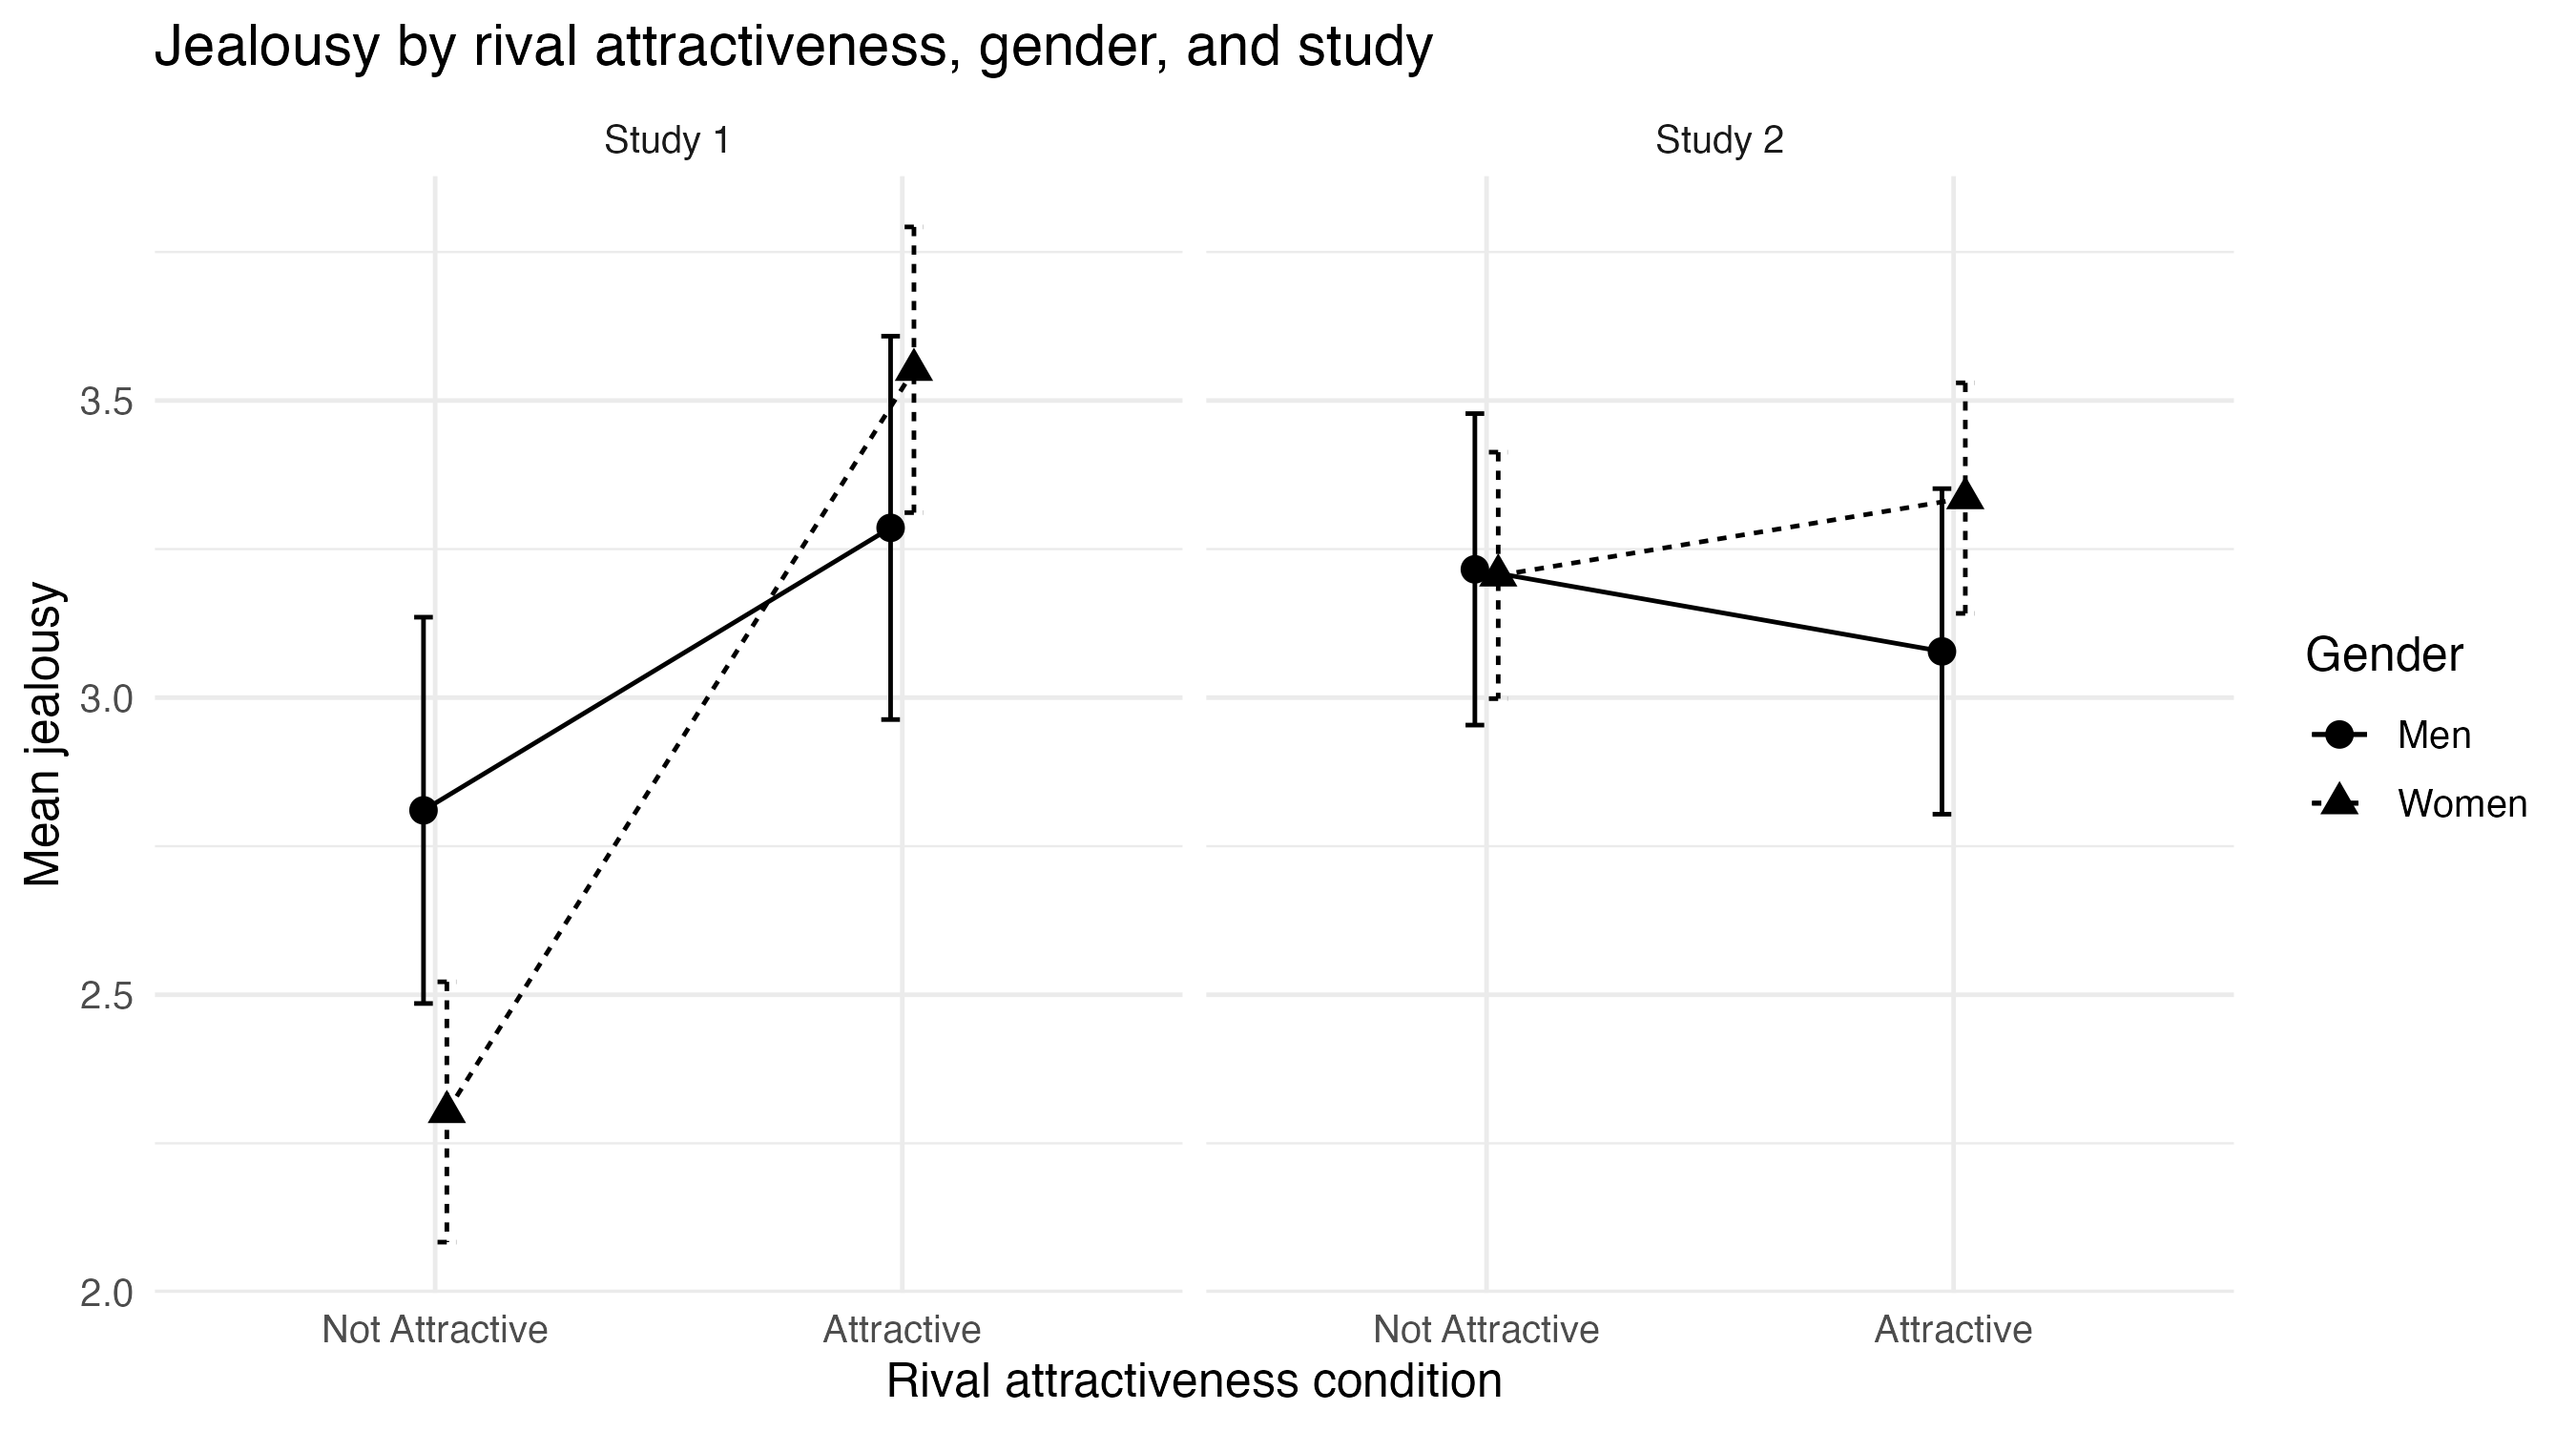
\includegraphics[width=0.8\textwidth]{extension_plot_main.png}
		\caption{Jealousy by rival attractiveness, gender, and study}
	\end{figure}
	
	\subsection{Ordered Logit Results}
	Figure 2 presents predicted probabilities of the highest jealousy category. Study 1 shows a clear increase for women when rivals are attractive, while Study 2 shows weaker effects.
	
	\begin{figure}[h]
		\centering
		
\includegraphics[width=0.8\textwidth]{ordered_logit_predicted_probability_plot.png}
		\caption{Predicted probability of highest jealousy category}
	\end{figure}
	
	\begin{table}[h]
		\centering
		\caption{Ordered Logit Interaction Results}
		\begin{table}

\caption{Ordered logit interaction results across studies}
\centering
\begin{tabular}[t]{llrrrr}
\toprule
Study & Term & Estimate & Std\_Error & t\_value & p\_value\\
\midrule
Study 1 & Attractive\_condition1:Gender1 & 0.2902458 & 0.1029849 & 2.818334 & 0.0048274\\
Study 2 & Attractive\_condition1:Gender1 & 0.0881862 & 0.0858699 & 1.026975 & 0.3044322\\
\bottomrule
\end{tabular}
\end{table}

	\end{table}
	
	\begin{table}[h]
		\centering
		\caption{Comparison of OLS and Ordered Logit Results}
		\begin{table}

\caption{Comparison of OLS and ordered logit interaction results}
\centering
\begin{tabular}[t]{lrrrr}
\toprule
Study & OLS\_F\_value & OLS\_p\_value & OrdLogit\_Estimate & OrdLogit\_p\_value\\
\midrule
Study 1 & 7.260610 & 0.0074036 & 0.2902458 & 0.0048274\\
Study 2 & 1.265632 & 0.2611847 & 0.0881862 & 0.3044322\\
\bottomrule
\end{tabular}
\end{table}

	\end{table}
	
	\section{Discussion and Conclusion}
	This replication confirms the original study’s findings only partially. The attractiveness-by-gender interaction is strong in Study 1 but weaker in Study 2. The ordered logit model supports similar conclusions but highlights variability across samples.
	
	Overall, the results suggest that the original effect is not fully robust. The extensions improve the analysis by testing stability across studies and across model specifications, providing a more nuanced understanding of the findings.
	
\end{document}